\part{Memory \& CPU}
\frame{\partpage}

\begin{frame}{Memory Hierarchy}
\begin{figure}
	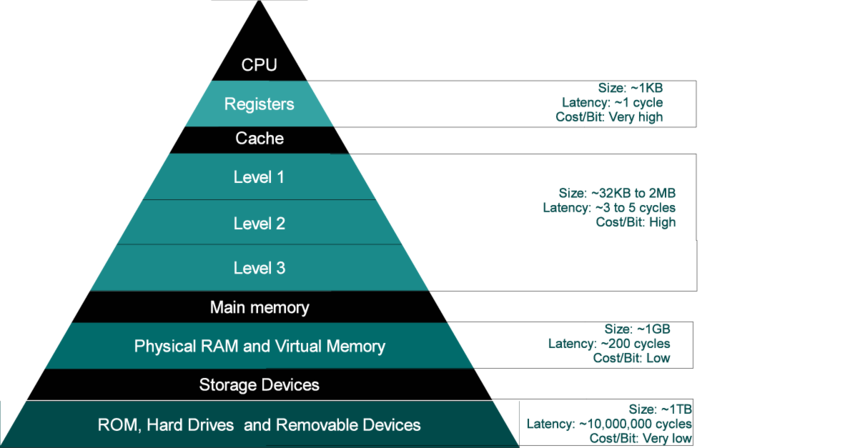
\includegraphics[width=1.0\textwidth,height=0.8\textheight]{Memory-hierarchy}  
\end{figure}
\end{frame}

\begin{frame}{Registers}
	\begin{itemize}
		\pause \item Registers are the only memory directly on the CPU
		\pause \item These tend to act as quick scratch pad for current calculations
		\pause \item Everything that the CPU operate on will get shifted into registers
		\pause \item Only issue it is slow to transfer data from RAM to registers
		\pause \item This is where the Cache comes in!  
	\end{itemize}
\end{frame}

\begin{frame}{Caches}
	\begin{itemize}
		\pause \item The cache acts as intermediate between the CPU and all off-board memory
		\pause \item There is usually different levels of cache, with different capabilities dependent on CPU e.g
		\pause \item Intel i-7 4770(Haswell)
		\begin{itemize}
			\pause \item L1 Data cache = 32KB with 4 cycles for simple access
			\pause \item L1 instruction cache = 32KB
			\pause \item L2 cache = 256KB with 12 cycles
			\pause \item L3 cache = 8MB with 26 cycles
		\end{itemize}
		\pause \item NB Ram typically takes 26 cycles + 57 nanoseconds to access 
	\end{itemize}
\end{frame}

\begin{frame}{Memory Optimisation}
	\begin{itemize}
		\pause \item Reduce Memory footprint
		\pause \item Write algorithms which reduce memory traversal
		\pause \item Increase cache hits
		\pause \item Increase temporal coherence
		\pause \item Utilise Pre-fetching
		\pause \item Avoid patterns which break caching 
	\end{itemize}
\end{frame}

\begin{frame}{Reduce Memory Footprint}
	\begin{itemize}
		\pause \item Consider use smaller data types
		\pause \item This will mean that your data structures will be more cache friendly
		\pause \item You can perhaps collapse several booleans into one integer and use bit flags 
	\end{itemize}
\end{frame}

\begin{frame}{Memory Alignment}
\begin{itemize}
	\pause \item The CPU will read memory aligned data much faster than non-aligned
	\pause \item Any \textit{N}-byte data is memory aligned if its starting address is evenly divisible by \textit{N}
	\pause \item e.g. A 32 bit integer is memory aligned if the starting address is 0x04000000, not 0x04000002
	\pause \item Make sure your structs or class has data types order highest to lowest  
\end{itemize}
\end{frame}

\begin{frame}{Avoiding Cache Misses}
	\begin{itemize}
		\pause \item The compiler and linker dictate how your code is laid out in memory
		\pause \item However the linker/compiler follows some simple rules
		\pause \item If you know these, then you can leverage them 
	\end{itemize}
\end{frame}

\begin{frame}{Compiler \& Linker rules}
\begin{itemize}
	\pause \item The machine code for a single function is contiguous in memory
	\pause \item Functions are laid out in memory in the order they appear in the cpp file
	\pause \item Function in the cpp are always contigous
\end{itemize}
\end{frame}

\begin{frame}{Applying Compiler \& Linker rules}
\begin{itemize}
	\pause \item Keep high performance code as small as possible
	\pause \item Avoid calling functions from a performance critical section of code
	\pause \item If you do have to call a function, place it as close as possible (never in another translation unit)
	\pause \item Use inline functions. Inlining a small function can lead to a performance boost. But this can lead to bloated code if over used (and lead to cache misses)
\end{itemize}
\end{frame}

\begin{frame}{Branch Prediction}
\begin{itemize}
	\pause \item CPUs will try to predict what branch to take ( if loop)
	\pause \item If the guess is wrong then we executed instructions that shouldn't have been called
	\pause \item This causes a stall, as the pipeline is flushed and the first instruction of the branch is then called
	\pause \item To solve this issue, you should attempt to reduce or remove all branches (see loop unrolling \& )
\end{itemize}
\end{frame}




